
\chapter{Results}
\label{ch:Results}



\section{Bertscore comparison}
\label{BertscoreComparison}

BERTScore is an evaluation metric for natural language generation tasks that leverages contextual embeddings from pre-trained language models such as BERT. Unlike traditional n-gram based metrics like BLEU or ROUGE, BERTScore computes similarity by aligning tokens in candidate and reference texts using the cosine similarity of their embeddings. This allows it to better capture semantic similarity even when surface forms differ. BERTScore has been shown to correlate strongly with human judgment across various NLP tasks~\cite{zhang2020bertscore}.


We compare sample results from TLDR application using \texttt{Llama-3.2-1B-Instruct-Q3\_K\_L} with \texttt{Chatgpt 4o}

\subsection{Result comparisons}
\label{subsec:Result comparisons}
\begin{itemize}
    \item \textit{97 Things Every Software Architect Should Know}
    \item \textit{Cracking the Coding Interview}
    \item \textit{189 Programming Questions and Solutions}
    \item \textit{System Design Interview: An Insider’s Guide} by Alex Xu
\end{itemize}

\textbf{TLDR Application:}
\\ \textbf{Note:} The references to the sources from TLDR's responses have been trimmed for comparison.

\begin{enumerate}[label=\arabic*.]

    
\item \textbf{User:} What is system design in software engineering?
\\ \textbf{Response:} System design is the process of creating a software system that meets the requirements of the users and the business. It involves defining the system architecture, selecting the appropriate technologies, and designing the user interface. The goal of system design is to create a system that is efficient, scalable, and maintainable. It is a critical process in software engineering that requires careful planning, analysis, and testing.



\item \textbf{User:} how to generate prime numbers?
\\ \textbf{Response:}
To generate prime numbers, you start with a list of all the numbers up to a certain number (in this case, max). Then, you cross off all the multiples of each prime number you find. This process continues until you've crossed off all the multiples of all the prime numbers you've found. The remaining numbers in the list are the prime numbers.
Here's a step-by-step guide:
1. Create a list of all the numbers up to max.
2. Cross off all the multiples of each prime number you find.
3. Continue this process until you've crossed off all the multiples of all the prime numbers you've found.
Note: You can use the Sieve of Eratosthenes algorithm to generate a list of prime numbers up to max.


\item \textbf{User:} what is caching?
\\ \textbf{Response:}
Caching is a technique used to improve the performance of an application by storing frequently accessed data in a temporary storage area, called the cache. This allows the application to retrieve the data quickly, reducing the load on the database or data store. Caching can be used to improve the performance of web applications, database applications, and even mobile applications. It is a technique that can be used to mitigate the problem of the "cold start" problem, where the application has to wait for the data to be retrieved from the database or data store. Caching can be implemented in various ways, including the use of caching tiers, caching strategies, and caching APIs.

\end{enumerate}

\textbf{ChatGPT:}
\\Note: The same documents mentioned earlier are uploaded to ChatGPT with this prompt: 'understand these documents and answer questions that i will ask based on them and keep the answer concise and precise'.

\begin{enumerate}[label=\arabic*.]

\item \textbf{User:} What is system design in software engineering? (use the previously attached documents as reference)
\\ \textbf{Response:} System design in software engineering is the process of defining the architecture, components, data flow, and interfaces of a software system to meet specified requirements. It focuses on how to build scalable, reliable, and maintainable systems by making high-level decisions on technologies, structure, and communication between parts of the system.



\item \textbf{User:} how to generate prime numbers? (use the previously attached documents as reference)
\\ \textbf{Response:}
To generate prime numbers, Cracking the Coding Interview outlines two primary methods: trial division and the Sieve of Eratosthenes. Trial division checks whether a number is divisible by any integer up to its square root and is suitable for verifying if a single number is prime. For generating multiple primes efficiently, the Sieve of Eratosthenes is recommended; it initializes a boolean array representing numbers up to a limit and iteratively marks multiples of each prime as non-prime, resulting in an array of prime indicators. This sieve approach offers better performance with a time complexity of O(n log log n), making it ideal for generating large sets of prime numbers.


\item \textbf{User:} what is caching?  (use the previously attached documents as reference)
\\ \textbf{Response:}
Caching, as described in System Design Interview: An Insider’s Guide and Cracking the Coding Interview, is a technique used to temporarily store frequently accessed or computationally expensive data in fast-access memory (typically RAM) to improve system performance and reduce load on backend systems like databases. It acts as an intermediary layer between clients and data stores, allowing applications to first check the cache for data before querying the database. Common strategies include read-through caching, expiration policies, and eviction methods like Least Recently Used (LRU), with considerations for consistency, fault tolerance, and scalability.

\end{enumerate}
\subsubsection{Quantitative comparison}
\label{subsubsec:tldrresultQuantitativecomparison}
The table below presents the precision, recall, and F1 score obtained using BERTScore \cite{bert-score}. These results are intended as illustrative examples, as the behavior and output of large language models (LLMs) can vary significantly and are not fully captured by a limited set of responses.

\begin{table}[h!]
\centering
\begin{tabular}{|c|c|c|c|}
\hline
\textbf{Row} & \textbf{Precision (P)} & \textbf{Recall (R)} & \textbf{F1 Score} \\
\hline
1 & 0.863623 & 0.897878 & 0.880417 \\
2 & 0.851684 & 0.854167 & 0.852923 \\
3 & 0.919073 & 0.916270 & 0.917669 \\
\hline
\end{tabular}
\caption{Performance metrics for three different evaluations}
\label{tab:metrics}
\end{table}
The results demonstrate a high degree of similarity between the model responses. Overall, the key takeaway is that the TLDR model is capable of generating responses that are comparable in quality to those produced by cloud-based models, despite operating with significantly fewer resources.
\section{Screenshots}
\label{SampleScreenshots}
\begin{figure}[h]
    \centering
    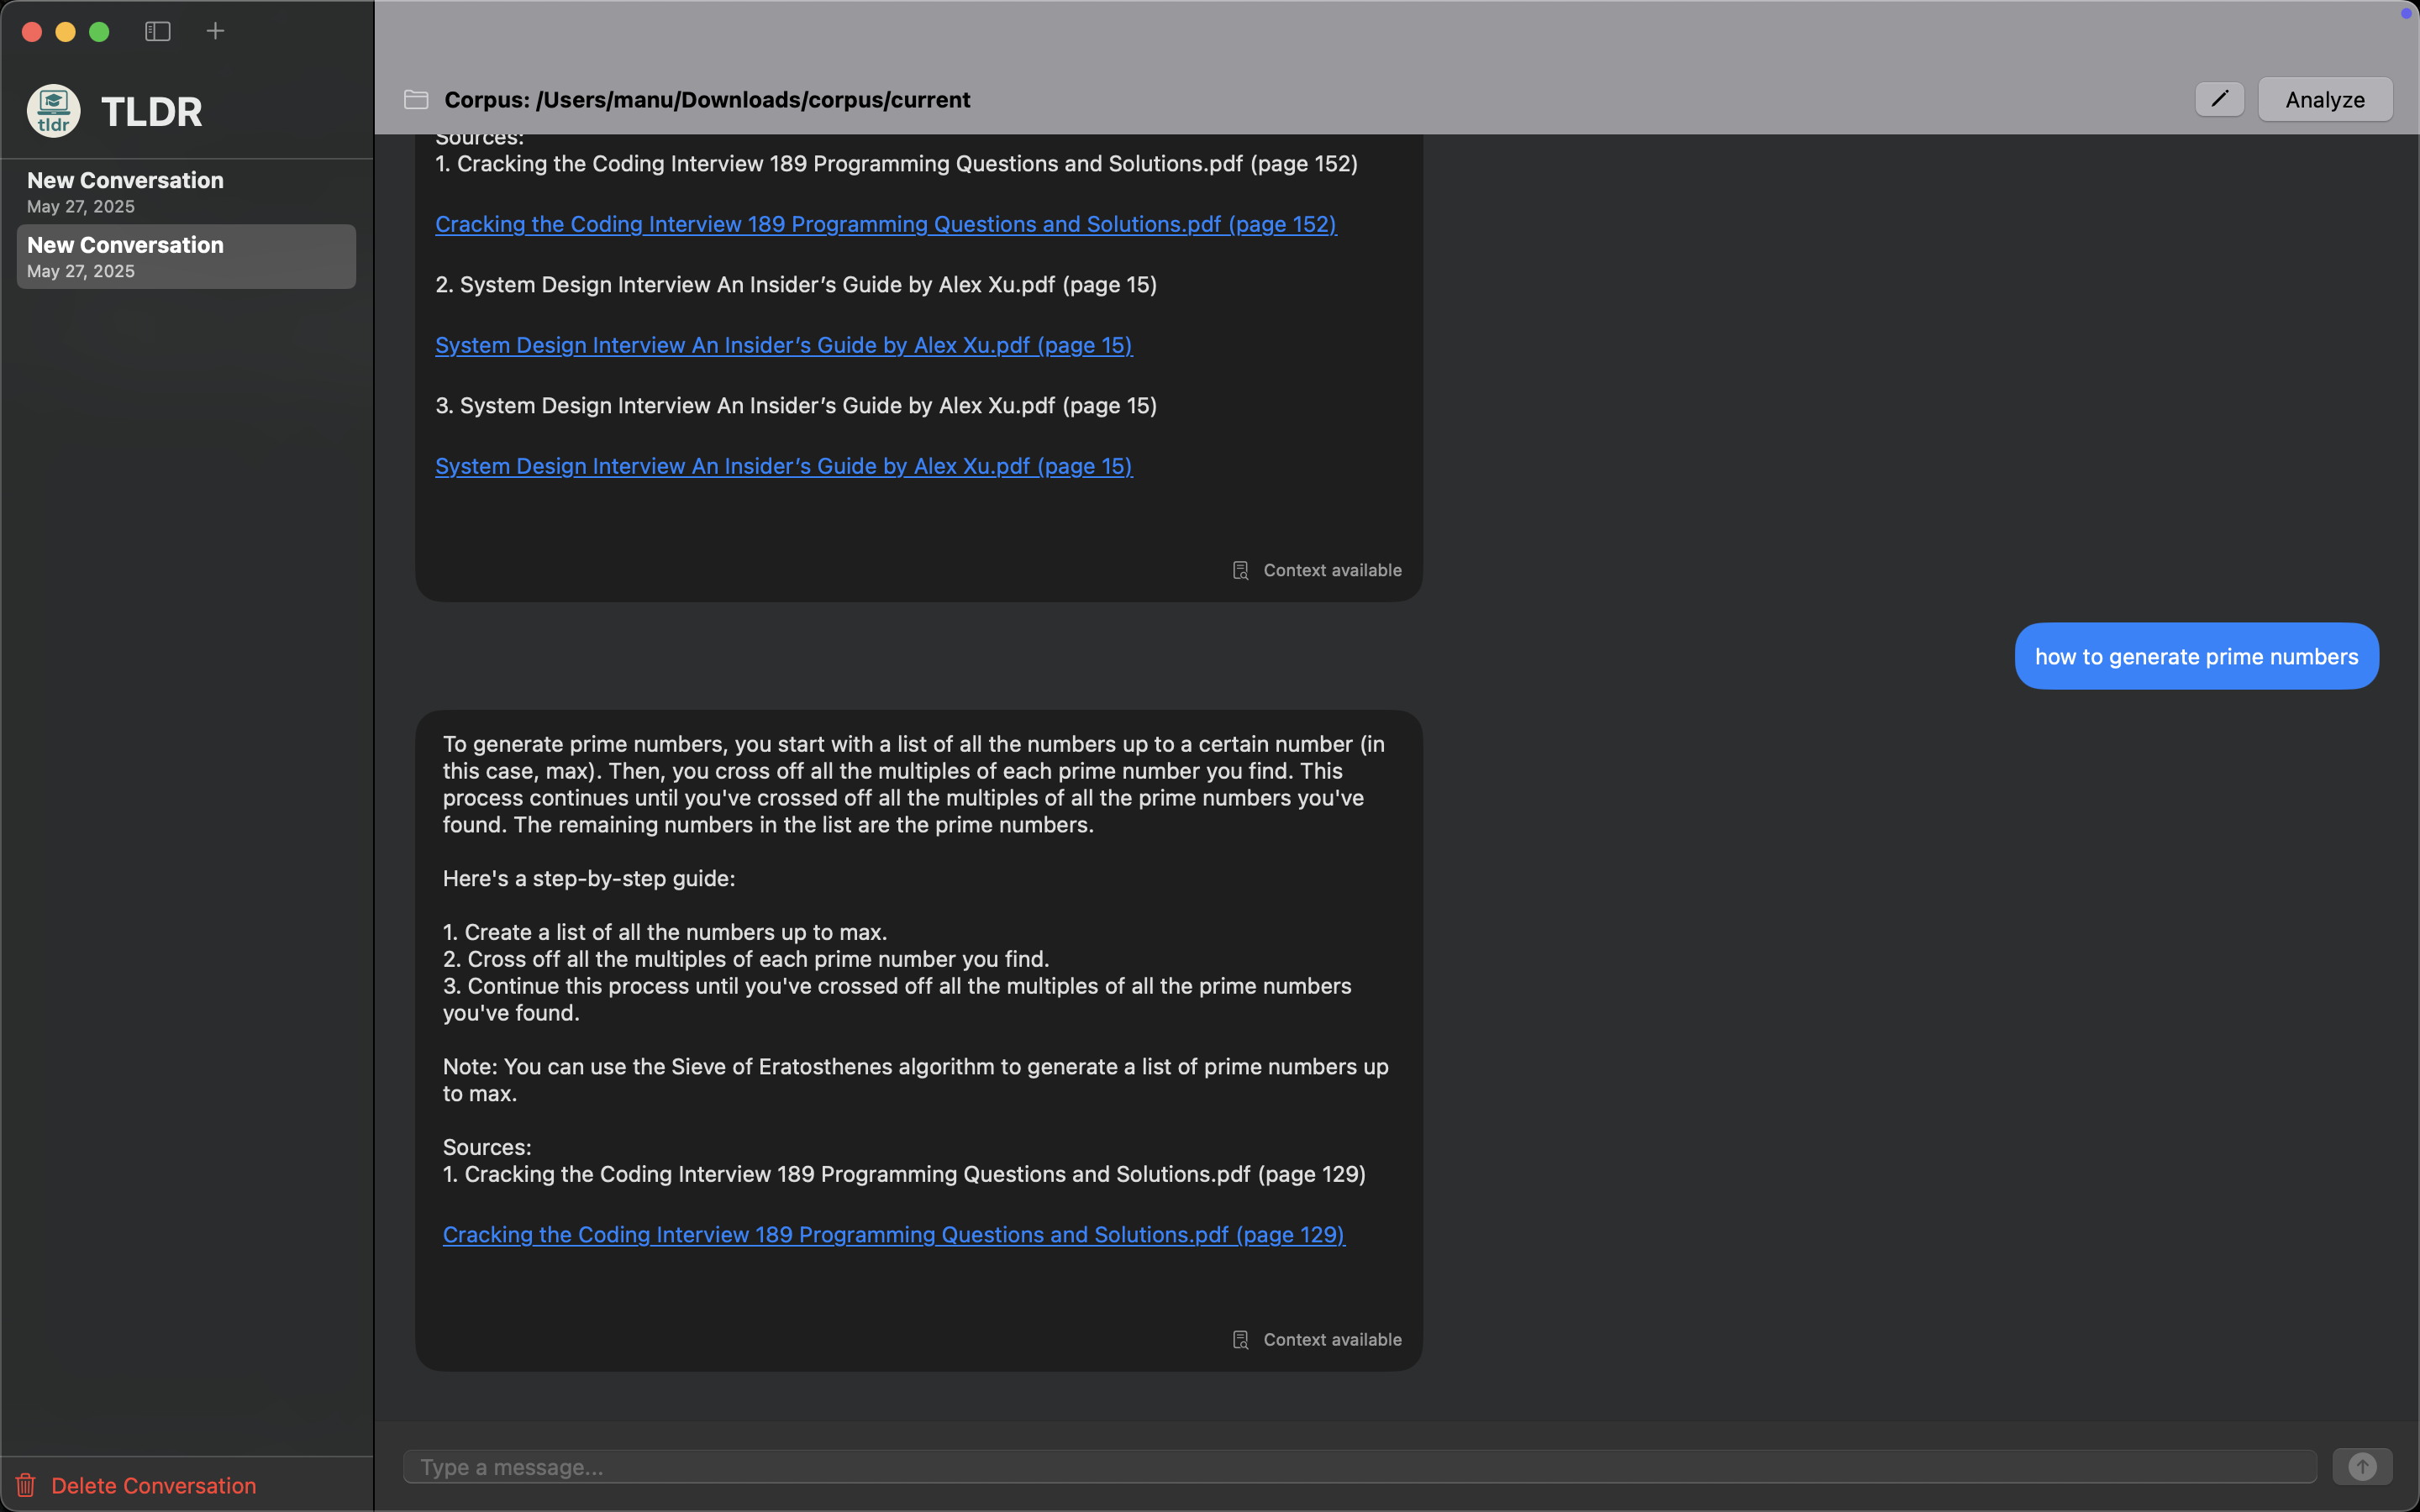
\includegraphics[width=1.0\linewidth]{images/result1.png}
    \caption{TLDR Application  Demonstration screenshot 1}
    \label{fig:tldrmodulesinteraction}
\end{figure}

\begin{figure}[h]
    \centering
    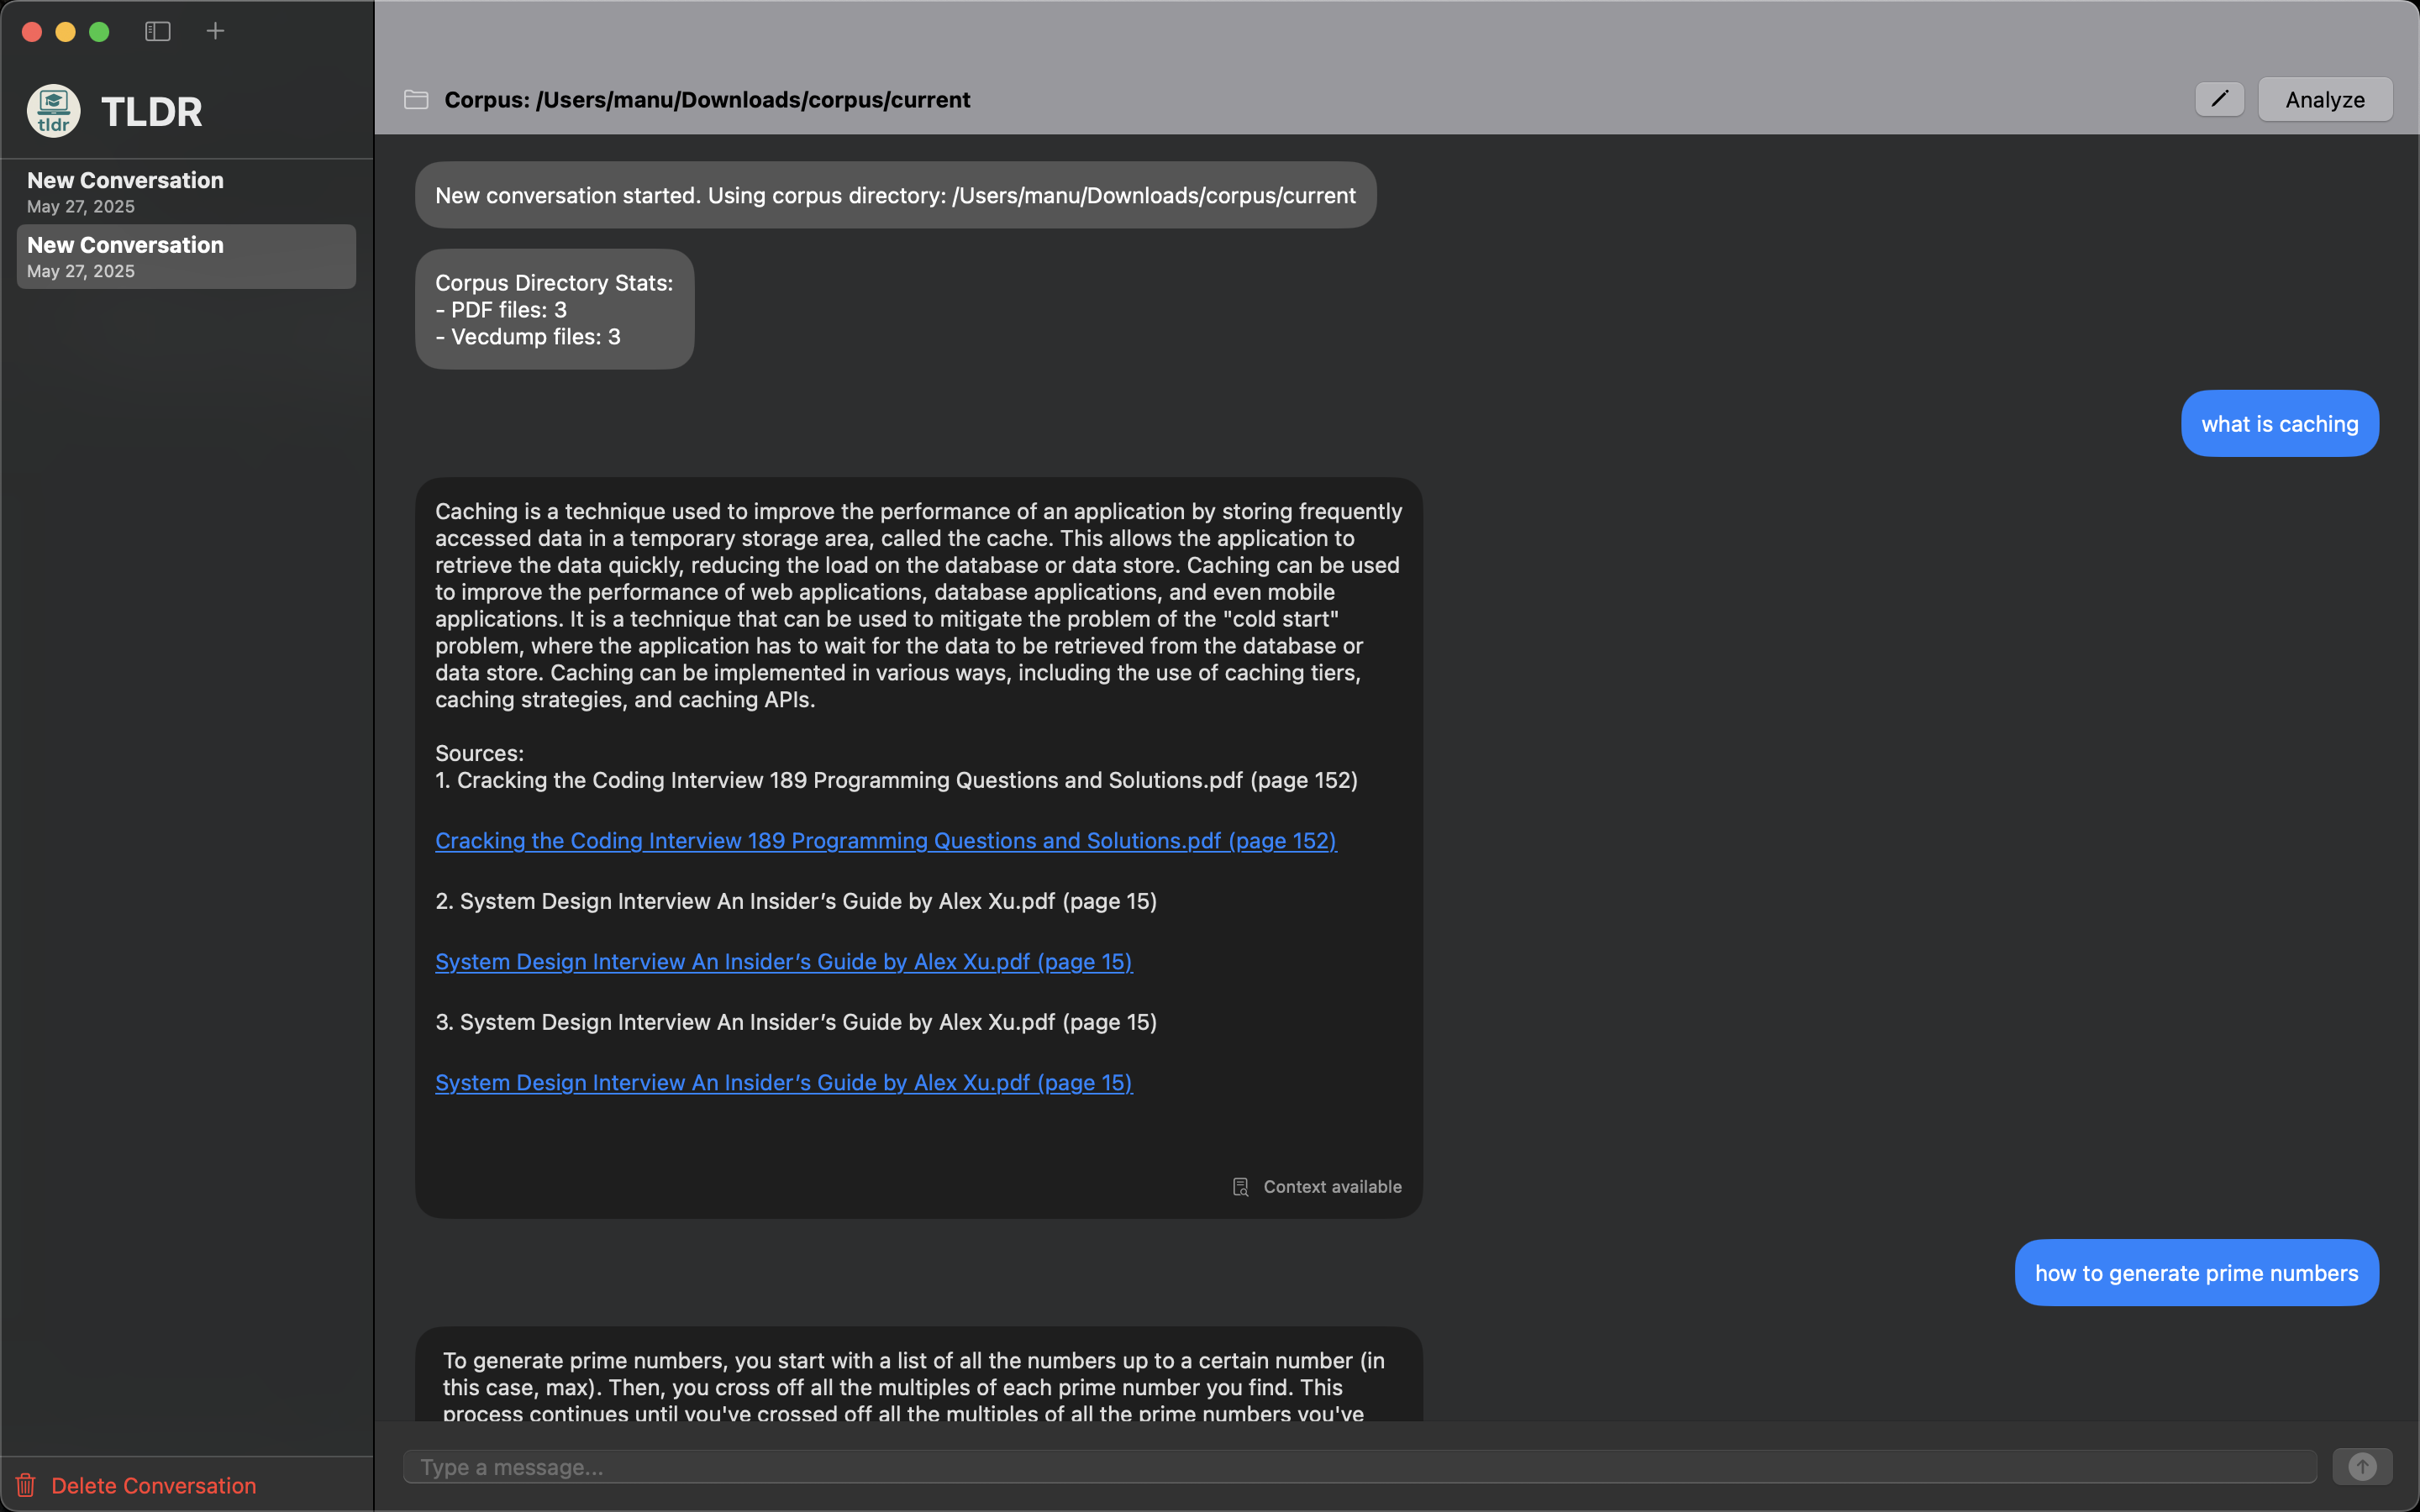
\includegraphics[width=1.0\linewidth]{images/result2.png}
    \caption{TLDR Application Demonstration screenshot 2}
    \label{fig:tldrmodulesinteraction}
\end{figure}

Simple Demo video: https://www.youtube.com/watch?v=KaDgJD-KyKA